\section{Containers}
\subsection{Übersicht}
\subsubsection{Sequence}
\begin{itemize}
	\item Reihenfolge bleibt erhalten
	\item find \chapref{find} in linearer Zeit
	\item array, vector, deque, list, forward\_list
\end{itemize}
\subsubsection{Associative}
\begin{itemize}
	\item Reihenfolge in sortierter Folge
	\item find \chapref{find} in logarithmischer Zeit
	\item map, multimap, set, multiset
\end{itemize}
\subsubsection{Hashed}
\begin{itemize}
	\item ohne Reihenfolge
	\item find \chapref{find} in konstanter Zeit
	\item unordered\_map, unordered\_multimap, \newline
		unordered\_set, unordered\_multiset
\end{itemize}
\subsubsection{Adaptors}
\begin{itemize}
	\item Provide a different interface for sequential containers. 
	\item stack, queue, priority\_queue
\end{itemize}
\subsection{Common API}
\begin{itemize}
	\item erease(iter)
	\item insert(iter,value)
	\item size(), empty()
	\item default-constructor
	\item copy-constructor
	\item equal-compare wenn Elemente gleicher Typ
	\item clear() $\rightarrow$ empty()
\end{itemize}
\subsubsection{Constructors}
	\begin{tabularx}{\columnwidth}{lX}
		Code & Bedeutung \\
		\hline
		C\{\} & Leerer Container besser als C() \\
		C\{e1,e2,\ldots,en\} & Mit \emph{initilizer list} initialisieren \\
		C\{n, e\} & Mit \emph{n} Kopien von \emph{e} initialisieren.  Besser C(n,e) verwenden, da sonst eine Mehrdeutigkeit ensteht, wenn \emph{n} ein gültiges Element des Containers ist (z.B. bei $vector<int>$) \\
		C\{ita, itb\} & Mit Elementen von iterator \emph{ita} bis ohne \emph{itb} initialisieren \\
	\end{tabularx}
	Beispiele:
\begin{lstlisting}
	std::vector<int> v{1,2,3,5,7,11};
	std::list<int>   l(5,42);
	std::deque<int>  q{v.begin(),v.end()};
\end{lstlisting}

\subsection{vector}
\begin{center}
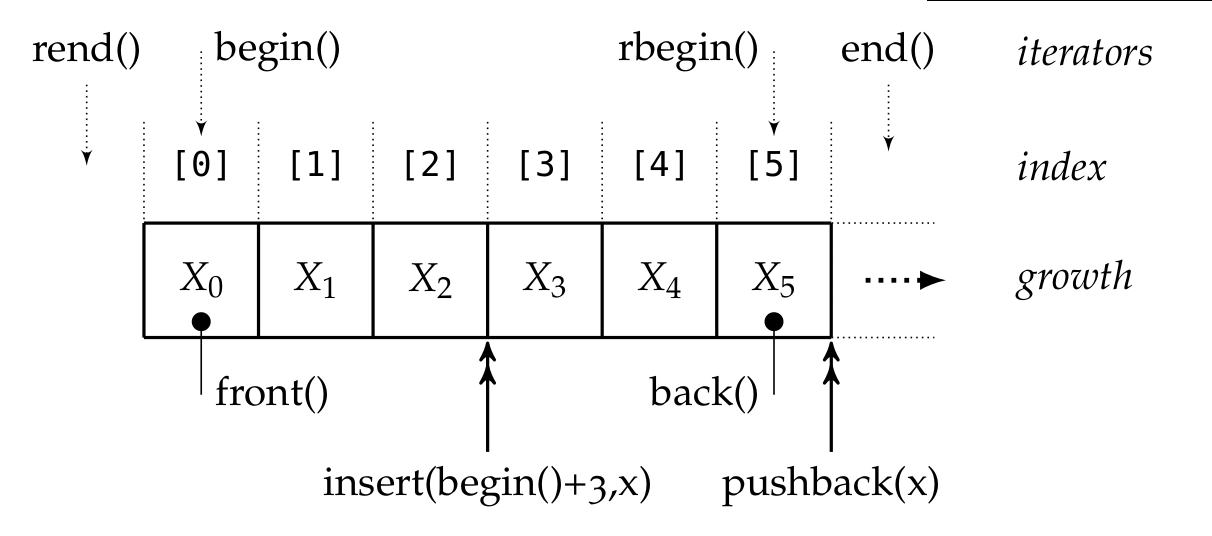
\includegraphics[width=\linewidth]{./bilder/iterators}
\end{center}
\begin{itemize}
\item Bool vector is bad because of premature optimization
\end{itemize}


\subsection{deque}
\begin{itemize}
\item push\_front
\end{itemize}

\subsection{array}
\begin{itemize}
\item similar to C-array, but keeps size
\end{itemize}

\subsection{list}
\begin{itemize}
\item fast insert
\end{itemize}
